\documentclass[xcolor=dvipsnames]{beamer}
\usepackage{xltxtra}
\usepackage[english]{babel}

\xdefinecolor{thecolor}{rgb}{0.5,0.0,0.5}

\mode<presentation>
{
	\usetheme{Rochester}
	\beamertemplatenavigationsymbolsempty
	\usecolortheme[named=thecolor]{structure}
	\setbeamercovered{transparent}
}

\title{Small Device C Compiler}
\subtitle{http://sdcc.sourceforge.net}

\author{Philipp Klaus Krause}

\subject{Small Device C Compiler, SDCC, C, STM8}

\begin{document}

\begin{frame}
	\titlepage
\end{frame}

\section{Small Device C Compiler}

\begin{frame}
	\frametitle{What is SDCC?}
	\begin{itemize}
		\item C compiler (ANSI C89, ISO C99, ISO C11, ISO C2X)
		\item Freestanding implementation or part of a hosted implementation
		\item Supporting tools (assembler, linker, simulator, ...)
		\item Works on many host systems (GNU/Linux, Windows, macOS, Hurd, OpenBSD, FreeBSD, ...)
		\item Targets various 8-bit architectures (MCS-51, DS80C390, Z80, Z180, eZ80 in Z80 mode, Rabbit 2000, Rabbit 2000A, Rabbit 3000A, SM83, TLCS-90, HC08, S08, STM8, pdk14, pdk15, pdk13, 6502, PIC14, PIC16)
		\item Has some unusual optimizations that make sense for these targets (in particular in register allocation)
		\item Users: µC programmers, and retrocomputing/-gaming developers
	\end{itemize}
\end{frame}

\begin{frame}
	\frametitle{Optimal Register Allocation in Polynomial Time}
	\begin{itemize}
		\item Register allocator based on graph-structure theory
		\item Optimal register allocation in polynomial time
		\item Flexible through use of cost function
		\item Provides substantial improvements in code quality
		\item Slow compilation for targets with many registers
		\item Compilation speed / code quality trade-off: --max-allocs-per-node
		\item Little-endian works better
	\end{itemize}
\end{frame}

\begin{frame}
	\frametitle{Bytewise Register Allocation and Spilling}
	\begin{itemize}
		\item Decide on the storage of variables bytewise
		\item Decide for each individual byte in a variable whether to store it in memory or a register
		\item Consider any byte of any register as a possible storage location
	\end{itemize}
\end{frame}

\begin{frame}
	\frametitle{SDCC vs.\ non-free compilers: STM8 Benchmark scores}
	\centerline{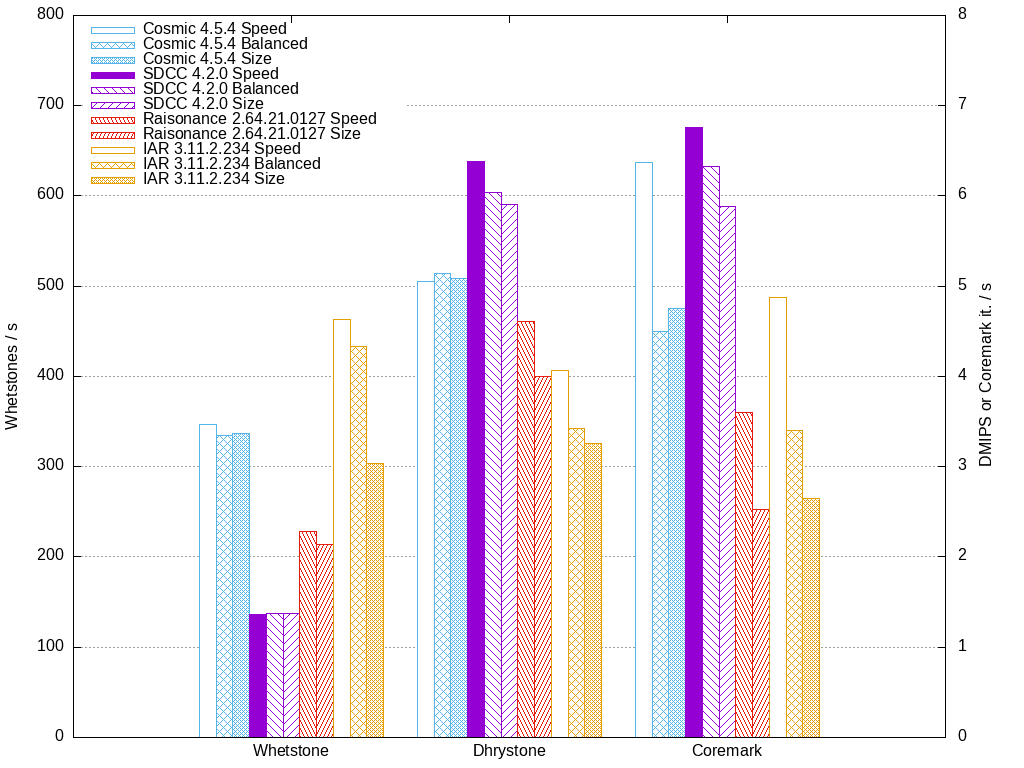
\includegraphics[scale=0.38]{scores-2022.png}}
\end{frame}

\begin{frame}
	\frametitle{SDCC vs.\ non-free compilers: STM8 Code size}
	\centerline{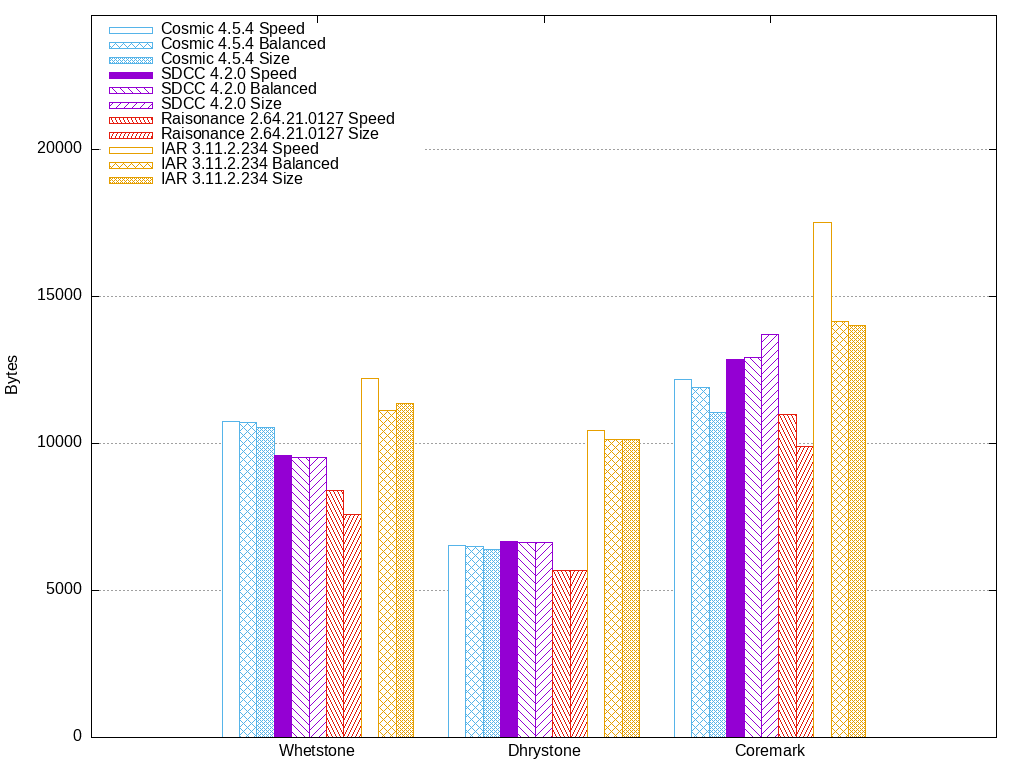
\includegraphics[scale=0.38]{sizes-2022.png}}
\end{frame}

\begin{frame}
	\frametitle{Regression testing}
	\begin{itemize}
		\item Regression testing of nightly snapshots
		\item $\approx 23000$ tests (twice as many as 2020) compiled and executed on simulators
		\item Tests mostly from fixed bugs and from GCC
		\item Targets architectures: MCS-51, DS390, Z80, Z180, eZ80 in Z80 mode, Rabbit 2000, Rabbit 3000A, LR35902, TLCS-90, HC08, S08, STM8, pdk14, pdk15
		\item Host OS: GNU/Linux, macOS, ``Windows'' (cross-compiled on GNU/Linux, tested via wine), FreeBSD
		\item Host architectures: x86, amd64, ppc, aarch64
	\end{itemize}
\end{frame}

\begin{frame}
	\frametitle{TODO}
	\begin{itemize}
		\item SDCC needs developers
		\item Fix SDCC bugs
		\item Improve SDCC further in standard compliance, optimizations, debug info, etc
		\item Improve IDE integration
		\item Improve hardware interface tools (Easy PDK programmer, free firmware for ST-Link, OpenRabbit, etc)
	\end{itemize}
\end{frame}

\end{document}

